\documentclass[aspectratio=169]{beamer}
\usepackage{hyperref}
\usepackage[T1]{fontenc}
\usepackage{tribhuvan}

% other packages
\usepackage{latexsym,amsmath,xcolor,multicol,booktabs,calligra}
\usepackage{graphicx,pstricks,listings,stackengine}
\usepackage{subcaption}
\usepackage{multirow}
\usepackage{bm}
\usepackage{booktabs}
\usepackage[brazil]{babel}  
\usepackage{siunitx}

\usepackage[backend=biber,style=numeric]{biblatex}
\addbibresource{references.bib}

\author{William de Oliveira}
\title[Introdução à Comunicação Científica e Projeto]{Estudo Numérico da Dinâmica de Corridas de Lama em Canal Aberto e Sua Interação com Obstáculos Submersos}
\subtitle{}
\institute{UFRGS | PROMEC | MEC-153}
\date{Janeiro, 2024}


% defs
\def\cmd#1{\texttt{\color{red}\footnotesize $\backslash$#1}}
\def\env#1{\texttt{\color{blue}\footnotesize #1}}
\definecolor{deepblue}{rgb}{0,0,0.5}
\definecolor{deepred}{rgb}{0.6,0,0}
\definecolor{deepgreen}{rgb}{0,0.5,0}
\definecolor{halfgray}{gray}{0.55}

\lstset{
    basicstyle=\ttfamily\small,
    keywordstyle=\bfseries\color{deepblue},
    emphstyle=\ttfamily\color{deepred},    % Custom highlighting style
    stringstyle=\color{deepgreen},
    numbers=left,
    numberstyle=\small\color{halfgray},
    rulesepcolor=\color{red!20!green!20!blue!20},
    frame=shadowbox,
}

% Notation:
\newcommand{\shearrate}{\dot{\gamma}}
\newcommand{\partialderiv}[2]{\frac{\partial #1}{\partial #2}}
\newcommand{\inlinepartialderiv}[2]{\nicefrac{\partial #1}{\partial #2}}
\newcommand{\velvector}{\bm{u}}
\newcommand{\viscosstresstensor}{\bm{\tau}}
\newcommand{\strainratetensor}{\bm{D}}
\newcommand{\stresstensor}{\bm{T}}
\newcommand{\xvelocity}{u}
\newcommand{\yvelocity}{v}
\newcommand{\zvelocity}{w}
\newcommand{\hb}{Herschel-Bulkley}
\newcommand{\yieldstress}{\tau_c}
\newcommand{\surftension}{\sigma_S}
\begin{document}

\begin{frame}
    \titlepage
    \vspace{-10pt}
    \begin{figure}
        \centering
        \begin{minipage}[c][0.2\textheight][c]{0.24\textwidth}
            \centering
            
\includegraphics[height=0.24\textheight]{images/logos/ufrgs.png}
        \end{minipage}
        \hfill
        \begin{minipage}[c][0.2\textheight][c]{0.24\textwidth}
            \centering
            
\includegraphics[height=0.18\textheight]{images/logos/promec.png}
        \end{minipage}
        \hfill
        \begin{minipage}[c][0.2\textheight][c]{0.24\textwidth}
            \centering
            
\includegraphics[height=0.16\textheight]{images/logos/capes.pdf}
        \end{minipage}
        \hfill
        \begin{minipage}[c][0.2\textheight][c]{0.24\textwidth}
            \centering
            
\includegraphics[height=0.10\textheight]{images/logos/reosul.png}
        \end{minipage}
    \end{figure}
\end{frame}

% \begin{frame}
    % \tableofcontents[sectionstyle=show,subsectionstyle=show/shaded/hide,subsubsectionstyle=show/shaded/hide]
% \end{frame}


\section{Introdução}

\subsection{Contextualização}

\begin{frame}{Contextualização}
    \begin{figure}
        \centering
        \includegraphics[width=0.5\textwidth]{../dissertation-project/fig/disasters_data/world_2000-2023_riskType.pdf}
        \caption{Quatro principais tipos de risco, em número de ocorrências, envolvendo
        desastres naturais, anos de 1900 a 2023. Dados de \cite{emdat_2023}.}
    \end{figure}
\end{frame}


\begin{frame}{Contextualização}
    \begin{figure}
        \centering
        \includegraphics[width=0.5\textwidth]{../dissertation-project/fig/disasters_data/world_accident_temperature_year.pdf}
        \caption{Número de deslizamento de terra e média da temperatura global. Dados de \cite{emdat_2023,NASA/GISS}}
    \end{figure}
\end{frame}

\begin{frame}{Contextualização}
    \begin{figure}
        \centering
        \includegraphics[width=0.75\textwidth]{../dissertation-project/fig/geospatial_maps/world_2000-2023_accidents_country_filtered.pdf}
        \caption{Número de desastres hidrológicos e geofísicos por país, anos 2000 a 2023. Dados de \cite{emdat_2023}}
    \end{figure}
\end{frame}

\begin{frame}{Contextualização}
    \begin{figure}
        \centering
        \includegraphics[width=0.6\textwidth]{../dissertation-project/fig/geospatial_maps/brazil_2000-2023_accidents_subtype_uf.pdf}
        \caption{Movimentos de Massa por estados no Brasil, anos 2000 a 2023. Dados de \cite{emdat_2023}}
    \end{figure}
\end{frame}

\begin{frame}{Contextualização}
    \begin{figure}
        \centering
        \begin{subfigure}{0.45\textwidth}
            \centering
            \includegraphics[width=\textwidth]{../dissertation-project/fig/disasters_data/rj_month_rain_massMovement.pdf}
            \caption{Rio de Janeiro.}
            \label{fig:rj}
        \end{subfigure}
        \hfill
        \begin{subfigure}{0.45\textwidth}
            \centering
            \includegraphics[width=\textwidth]{../dissertation-project/fig/disasters_data/sp_month_rain_massMovement.pdf}
            \caption{São Paulo.}
            \label{fig:sp}
        \end{subfigure}
    
        \caption{Movimentos de massa e índice pluviométrico. Dados dos acidentes de \cite{atlas_brazil_2023}, anos de 1931 a 2023. Dados climatológicos de \cite{ANA}, anos de 1931 a 2020.}
        \label{fig:test}
    \end{figure}
\end{frame}




% ---------------------------------------------------------------------------------------------------- %
\subsection{Objetivos}

\begin{frame}{Objetivos}
asdf
\end{frame}
% ---------------------------------------------------------------------------------------------------- %

\subsection{Organização do Trabalho}

\begin{frame}{Frame Title}
    \begin{itemize}
        \item This template is modified from Tsinghua University's Beamer template: \url{https://www.overleaf.com/latex/templates/thu-beamer-theme/vwnqmzndvwyb} \pause
        \item The original template is modified from \newline \url{https://www.latexstudio.net/archives/4051.html}
        \item The real original template is not found \cite{origin}.
    \end{itemize}
\end{frame}

\section{Fundamentação}

\subsection{Movimentos de Massa}
% \begin{frame}{Movimentos de Massa}
%     \begin{exampleblock}{\Large Tipos de movimentos}
%         \begin{itemize}
%             \Large
%             \item Desmoronamentos;
%             \item Tombamentos;
%             \item Deslizamento de terra;
%             \item Corridas detríticas;
%             \item Corridas de lama.
%         \end{itemize}
%     \end{exampleblock}
% \end{frame}

\begin{frame}{Movimentos de Massa}
    \begin{minipage}[c]{0.70\textwidth}
        \centering
        \includegraphics[width=\textwidth]{../dissertation-project/fig/diagrams/rheological_classification_english.pdf}
    \end{minipage}
    \hfill    
    \begin{minipage}[c]{0.28\textwidth}
        \captionof{figure}{Classificação dos movimentos de massa em encostas íngremes, como função
        da porção sólida e do tipo de material. Adaptado de \cite{coussot_recognition_1996}.}
    \end{minipage}
\end{frame}

\begin{frame}{Movimentos de Massa}
    \begin{table}[ht]
        \centering
        \captionof{table}{Magnitude e mobilidade dos movimentos de massa\footnote{Fonte: \cite{takahashi_debris_2014}}.}
        \small
        \begin{tabular}{lccc}
                \hline
                Fenômeno                & Volume deslocado                                             & Velocidade                             & Distância máxima \\
                                        & (\SI{}{\cubic\meter})                                & (\unit[per-mode = symbol]{\metre\per\second})                                 & (\SI{}{\kilo \meter})             \\ \hline
                Deslizamento de terra   & 10 $\sim$ 10\textsuperscript{6}                       & 10\textsuperscript{-6} $\sim$ 10       & $<$ 0,3          \\
                Desmoronamento          & 2 $\times$ 10\textsuperscript{5}                      & \textemdash                                     & 0,7              \\
                Corridas Detríticas     & 10\textsuperscript{3} $\sim$ 10\textsuperscript{6}    & 0,5 $\sim$ 20                          & 0,2 $\sim$ 10    \\
                Avalanches Detríticas   & 10\textsuperscript{7} $\sim$ 10\textsuperscript{10}   & 10 $\sim$ 10\textsuperscript{2}        & < 30             \\
                    \hline
            \end{tabular}
            \label{tab:mov_massa_magnitude}
        \end{table}
\end{frame}



\subsection{Escoamento em Canais}

\begin{frame}{Escoamento em canais}
    \begin{minipage}[c]{0.56\textwidth}
        \begin{exampleblock}{Canal aberto (superfície livre)}
            \centering
            \includegraphics[width=\textwidth]{../dissertation-project/fig/diagrams/channel_section.pdf}
            \captionof{figure}{Diagrama com seção transversal de um canal genérico.}           
        \end{exampleblock}
    \end{minipage}
    \hfill
    \pause
    \begin{minipage}[c]{0.36\textwidth}
        \begin{exampleblock}{Seção Retangular}
            \centering
            \includegraphics[width=0.5\textwidth]{../dissertation-project/fig/diagrams/cross_section_rectangular.pdf}
            \captionof{figure}{Seção canal retangular.}    
        \end{exampleblock}
        \begin{exampleblock}{Raio hidráulico}
            \begin{equation}
                R_h = \frac{Bh}{B+2h}
            \end{equation}
        \end{exampleblock}
    \end{minipage}
\end{frame}

\begin{frame}{Adimensionais}
    \begin{exampleblock}{Número de Froude}
        \begin{equation}
            Fr = \frac{U}{\sqrt{gh}} 
            = \frac{\text{Forças Inerciais}}{\text{Forças Gravitacionais}}
        \end{equation}        
    \end{exampleblock}

    \begin{exampleblock}{Número de Reynolds}
        \begin{equation}
            Re = \frac{\rho U L}{\mu} = \frac{4UR_h}{\nu} 
            = \frac{\text{Forças Inerciais}}{\text{Forças Viscosas}}
        \end{equation}        
    \end{exampleblock}
\end{frame}



\subsection{Reologia}

\begin{frame}{Reologia}
    \includegraphics[width=\textwidth]{../dissertation-project/fig/diagrams/fluid_classification.pdf}
    \captionof{figure}{Fluidos não newtonianos. (a) Curvas se fluidos
    viscoplásticos. (b) Fluidos Puramente Viscosos. (c) Teste de taxa de deformação
    constante.}
\end{frame}

\begin{frame}{Reologia}
    \centering
    \includegraphics[width=0.65\textwidth]{../dissertation-project/fig/diagrams/water-debris_classification.pdf}
    \captionof{figure}{Classificação reológica de misturas de água e detritos. Adaptado de \cite{coussot_1997_mudflow}.}
\end{frame}

\subsection{Equacionamento}
\begin{frame}
    \begin{exampleblock}{Conservação da Massa}
        \begin{equation}
            \partialderiv{\rho}{t} + \nabla \cdot \rho \bm{u} = 0
        \end{equation}
    \end{exampleblock}

    \begin{exampleblock}{Conservação de \textit{Momentum}}
        \begin{equation}
            \rho \left( \partialderiv{\bm{u}}{t}  + \bm{u} \cdot \nabla \bm{u} \right) =
            \bm{b} + \nabla \cdot \bm{T}
        \end{equation}
    \end{exampleblock}

    \hspace{0.5cm} Definindo o tensor de tensão como $\bm{T} = -p\bm{I} + \bm{\tau}$ e a 
    aceleração gravitacional como a única força externa aplicada ao fluido:
        \vspace{0.25cm}
        \begin{equation}
            \rho \left( \partialderiv{\bm{u}}{t}  + \bm{u} \cdot \nabla \bm{u} \right) =
            -\nabla p + \nabla \cdot \bm{\tau} + \rho \bm{g}
        \end{equation}
\end{frame}

\begin{frame}
    \hspace{0.5cm} Em regime permanente, a equação de \textit{momentum} fica:
    \begin{equation}
        \begin{split}
            \partialderiv{\tau}{y} + \rho g \sin{\theta} &= 0 \\
            -\partialderiv{p}{y} - \rho g \cos{\theta} &= 0
        \end{split}
        \label{eq:motion_steady_state_partial}
    \end{equation}

    \hspace{0.5cm} Integrando e usando as condições de contorno da superfície livre e não deslizamento na parede:
    \begin{equation}
        \begin{split}
            u(y) &= \frac{\alpha}{m+1} \left[y_0^{(m+1)} - {(y_0-y)}^{(m+1)}\right]
            \hspace{0.5cm} \text{quando} \hspace{0.5cm} y \leq y_0
            \\
            u(y) &= u(y_0) = \frac{\alpha}{m+1} \left[ y_0^{(m+1)} \right]
            \hspace{1.9cm} \text{quando} \hspace{0.5cm} h \geq y \geq y_0
        \end{split}
        \label{eq:velocity_distribution}
    \end{equation}
    
    com $m=\frac{1}{n}$, $y_0 = h - \frac{\yieldstress}{\rho g \sin{\theta}}$ e $\alpha = \left({\frac{\rho g \sin{\theta}}{K}}\right)^m$.
\end{frame}

\begin{frame}
    \begin{minipage}[c]{0.65\textwidth}
        \begin{exampleblock}{Perfil de velocidade de um fluido tipo HB}
            \centering
            \includegraphics[width=0.85\textwidth]{../dissertation-project/fig/diagrams/HB_velocity-distribution_inclined-plane.pdf}
            \captionof{figure}{Distribuição de velocidade ao longo da seção transversal, para diferentes valores de $n$. Adaptado de \cite{coussot_1997_mudflow}.}
        \end{exampleblock}
    \end{minipage}
    \hfill
    \begin{minipage}[t]{0.32\textwidth}
        \small
        \begin{equation}
            \begin{split}
                U &= \frac{u(y)}{u(y_0)} \\
                Y &= \frac{y}{y_0} \\
                G &= \frac{\rho g \sin{\theta}}{\yieldstress}
            \end{split}
            \label{eq:dimensionaless_velocity_distribution}
        \end{equation}        
    \end{minipage}
\end{frame}

\subsection{Adimensionais}

\begin{frame}

    \begin{exampleblock}{Modelo de fluido tipo HB}
        \begin{equation}
            \label{eq:HB_shear_stress}
            \begin{split}
                \tau &= \yieldstress + K \shearrate^n
                \text{ ,\hspace{0.5 cm} quando \hspace{0.2cm}} \shearrate = \partialderiv{u}{y} \ne 0
                \\
                |\tau| &\leq \yieldstress
                \text{ ,\hspace{1.65cm} quando \hspace{0.2cm}} \shearrate = 0
            \end{split}
        \end{equation}
    \end{exampleblock}

    \begin{exampleblock}{Reynolds canal aberto, fluido tipo HB}
        \begin{equation}
            Re_{HB} = \frac{8 \rho U^2}{\tau_c + K \left( \frac{2U}{R_h} \right)^n}
        \end{equation}
    \end{exampleblock}

\end{frame}

% \section{Reologia}

\begin{frame}{Examples}
    \begin{exampleblock}{Numbered Equation}
        \begin{equation} % Add * to remove numbering
            J(\theta) = \mathbb{E}_{\pi_\theta}[G_t] = \sum_{s\in\mathcal{S}} d^\pi (s)V^\pi(s)=\sum_{s\in\mathcal{S}} d^\pi(s)\sum_{a\in\mathcal{A}}\pi_\theta(a|s)Q^\pi(s,a)
        \end{equation}
    \end{exampleblock}
    \begin{exampleblock}{Multi-line Equation\footnote{This is a footnote}}
        % Use & to separate
        \begin{align}
            Q_\mathrm{target}&=r+\gamma Q^\pi(s^\prime, \pi_\theta(s^\prime)+\epsilon)\\
            \epsilon&\sim\mathrm{clip}(\mathcal{N}(0, \sigma), -c, c)\nonumber
        \end{align}
    \end{exampleblock}
\end{frame}

\begin{frame}
    \begin{exampleblock}{Numbered Multi-line Equation}
        % Taken from Mathmode.tex
        \begin{multline}
            A=\lim_{n\rightarrow\infty}\Delta x\left(a^{2}+\left(a^{2}+2a\Delta x+\left(\Delta x\right)^{2}\right)\right.\label{eq:reset}\\
            +\left(a^{2}+2\cdot2a\Delta x+2^{2}\left(\Delta x\right)^{2}\right)\\
            +\left(a^{2}+2\cdot3a\Delta x+3^{2}\left(\Delta x\right)^{2}\right)\\
            +\ldots\\
            \left.+\left(a^{2}+2\cdot(n-1)a\Delta x+(n-1)^{2}\left(\Delta x\right)^{2}\right)\right)\\
            =\frac{1}{3}\left(b^{3}-a^{3}\right)
        \end{multline}
    \end{exampleblock}
\end{frame}

\begin{frame}{Graph and Columns}
    % From thuthesis user guide.
    %\begin{minipage}[c]{0.3\linewidth}
     %   \psset{unit=0.8cm}
      %  \begin{pspicture}(-1.75,-3)(3.25,4)
       %     \psline[linewidth=0.25pt](0,0)(0,4)
        %    \rput[tl]{0}(0.2,2){$\vec e_z$}
         %  \rput[tl]{0}(2.8,-1.1){$\vec C_{ptm{ext}}$}
          %  \rput[br]{0}(-0.3,2.1){$\theta$}
           % \rput{25}(0,0){%
            %\psframe[fillstyle=solid,fillcolor=lightgray,linewidth=.8pt](-0.1,-3.2)(0.1,0)}
            %\rput{25}(0,0){%
            %\psellipse[fillstyle=solid,fillcolor=yellow,linewidth=3pt](0,0)(1.5,0.5)}
            %\rput{25}(0,0){%
            %\psframe[fillstyle=solid,fillcolor=lightgray,linewidth=.8pt](-0.1,0)(0.1,3.2)}
            %\rput{25}(0,0){\psline[linecolor=red,linewidth=1.5pt]{->}(0,0)(0.,2)}
%           \psRotation{0}(0,3.5){$\dot\phi$}
%           \psRotation{25}(-1.2,2.6){$\dot\psi$}
            %\psline[linecolor=red,linewidth=1.25pt]{->}(0,0)(0,2)
%            \psline[linecolor=red,linewidth=1.25pt]{->}(0,0)(3,-1)
 %           \psline[linecolor=red,linewidth=1.25pt]{->}(0,0)(2.85,-0.95)
  %          \psarc{->}{2.1}{90}{112.5}
   %         \rput[bl](.1,.01){C}
    %    \end{pspicture}
    %\end{minipage}
    \hspace{1cm}
    \begin{minipage}{0.5\linewidth}
        \medskip
        %\hspace{2cm}
        \begin{figure}[h]
            \centering
            \includegraphics[height=.4\textheight]{images/dtmf.pdf}
        \end{figure}
    \end{minipage}
    \end{frame}

\begin{frame}[fragile]{Common \LaTeX{} Commands}
    \begin{exampleblock}{Commands}
        \centering
        \footnotesize
        \begin{tabular}{llll}
            \cmd{chapter} & \cmd{section} & \cmd{subsection} & \cmd{paragraph} \\
            Chapter & Section & Subsection & Paragraph \\\hline
            \cmd{centering} & \cmd{emph} & \cmd{verb} & \cmd{url} \\
            Centering & Emphasis & Verbatim & URL \\\hline
            \cmd{footnote} & \cmd{item} & \cmd{caption} & \cmd{includegraphics} \\
            Footnote & Item & Caption & Graphics \\\hline
            \cmd{label} & \cmd{cite} & \cmd{ref} \\
            Label & Cite & Reference\\\hline
        \end{tabular}
    \end{exampleblock}
    \begin{exampleblock}{Environments}
        \centering
        \footnotesize
        \begin{tabular}{lll}
            \env{table} & \env{figure} & \env{equation}\\
            Table & Figure & Equation \\\hline
            \env{itemize} & \env{enumerate} & \env{description}\\
            Unnumbered List & Numbered List & Description \\\hline
        \end{tabular}
    \end{exampleblock}
\end{frame}

\section{Escoamento Sobre Estrutura}

% \begin{frame}{Características}
%     \Large
%     \begin{itemize}
%         \item Escoamento uniforme;
%         \item Escoamento laminar;
%         \item Superfície livre;
%         \item Canal infinitamente largo.
%     \end{itemize}
% \end{frame}

\subsection{Escoamento Sobre Estrutura}

\begin{frame}{Definição do Problema}
    \begin{minipage}[c]{0.49\textwidth}
        \begin{exampleblock}{Plano inclinado, bidimensional}
            \includegraphics[width=\textwidth]{../dissertation-project/fig/diagrams/free-surface_inclined-plane.pdf}
            \captionof{figure}{Escoamento de superfície livre de altura $h$ em um plano infinitamente largo, com
            velocidade uniforme.}
        \end{exampleblock}
    \end{minipage}
    \hfill
    \begin{minipage}[c]{0.49\textwidth}
        \begin{exampleblock}{Plano inclinado, "tridimensional"}
            \includegraphics[width=\textwidth]{../dissertation-project/fig/diagrams/free-surface-obstacle.pdf}
            \captionof{figure}{Escoamento incidindo sobre um corpo submerso retangular ao fundo do canal, com velocidade $u(y)$.}
        \end{exampleblock}
    \end{minipage}
\end{frame}

\begin{frame}{Literatura}
    
    \begin{exampleblock}{\Citeauthor{Forbes1982} (1982)}
        \begin{itemize}
            \item Modelo numérico, bidimensional;
            \item Fluido invíscido e incompressível;
            \item Mecanismo de geração de ondas.
        \end{itemize}
    \end{exampleblock}

    \begin{exampleblock}{\Citeauthor{Lawrence1987} (1987)}
        \begin{itemize}
            \item Aparato experimental, obstáculo fixo e submerso;
            \item Regimes hidráulicos dependentes de perturbação/formação escoamento.
        \end{itemize}
    \end{exampleblock}

\end{frame}

\begin{frame}{Literatura}
    \begin{exampleblock}{\Citeauthor{Vanden-Broeck1987} (1987); 
        \Citeauthor{King1987} (1987); \Citeauthor{Forbes1988} (1988)}
        \begin{itemize}
            \item Fluidos ideais;
            \item Obstáculos de diferentes formatos;
            \item Variação do número de Froude caracterizando o regime hidráulico.
        \end{itemize}
    \end{exampleblock}

    \begin{exampleblock}{\Citeauthor{Fadda1997} (1997)}
        \begin{itemize}
            \item Numérico e experimental;
            \item Dimensão característica do obstáculo;
            \item Variações de vazão, influência do número de Reynolds.
        \end{itemize}
    \end{exampleblock}
\end{frame}

\begin{frame}{Literatura}
    \begin{exampleblock}{\Citeauthor{Bush1994} (1994); \Citeauthor{Singh2000} (2000)}
        \begin{itemize}
            \item Fluidos viscoelásticos;
            \item Sedimentação em diferentes fluidos.
        \end{itemize}
    \end{exampleblock}

    \begin{exampleblock}{\Citeauthor{Bernabeu2018} (2018); \Citeauthor{Hinton2023} (2023)}
        \begin{itemize}
            \item Fluido viscoplástico;
            \item Reologias mais complexas;
            \item Parâmetros do fluido influenciando a dinâmica do escoamento.
        \end{itemize}
    \end{exampleblock}
\end{frame}


% \begin{frame}{Literatura}
%     \begin{minipage}[c]{0.49\textwidth}
%         \begin{exampleblock}{Primeiros estudos}
%             \begin{itemize}
%                 \item Validação de modelos lineares;
%                 \item Fluidos invíscidos, escoamento potencial;
%                 \item Domínio bidimensional;
%                 % \item Estudos numérico/experimental;
%                 \item Forma e disposição de obstáculos.
%             \end{itemize}
%         \end{exampleblock}
%     \end{minipage}
%     \hfill
%     \begin{minipage}[c]{0.49\textwidth}
%         \begin{exampleblock}{Trabalhos mais recentes}
%             \begin{itemize}
%                 \item Regimes hidráulicos subcrítico, crítico e supercrítico;
%                 % \item Avaliações numéricas/experimental;
%                 \item Aplicação de fluidos não newtonianos;
%                 \item Zonas de estagnação da velocidade;
%                 \item Efeitos dinâmicos do escoamento.
%             \end{itemize}
%         \end{exampleblock}
%     \end{minipage}
        
% \end{frame}

% \begin{frame}{Tópicos de Análise}
%     \begin{itemize}
%         \large
%         \item Comportamento da superfície livre;
%         \item Variação da vazão e seus efeitos na dinâmica do escoamento;
%         \item Coeficientes de arrasto e sustentação sob diferentes cenários;
%         \item Avaliação dos esforços induzidos no obstáculo submerso;
%         \item Influência da região de estagnação do escoamento;
%         \item Números de Reynolds e de Froude para caracterizar o escoamento.
%     \end{itemize}
% \end{frame}

\section{Metodologia Numérica}

\begin{frame}
    \begin{exampleblock}{Metodologia Numérica}
        \begin{itemize}
            \item Método dos Volumes Finitos;
            \item OpenFOAM + cfMesh;
            \item Método VOF;
            \item Modelo bi-viscoso;
            \item interFoam solver;
            \item Automatização Python e Bash.
        \end{itemize}
    \end{exampleblock}
\end{frame}

% \begin{frame}{Método VOF}
%     O método Volume de Fluido, no inglês \textit{Volume of Fluid} (VOF), é usado para capturar a superfície livre do escoamento. A dependência temporal da fase $\alpha$, para um problema bidimensional, é governada pela Eq.~\ref{eq:alpha_phase}.

%     \begin{equation} \label{eq:alpha_phase}
%         \partialderiv{\alpha}{t} + u \partialderiv{\alpha}{x} + v \partialderiv{\alpha}{y} = 0
%     \end{equation}

% \end{frame}

\begin{frame}{Método VOF} 
    \centering
    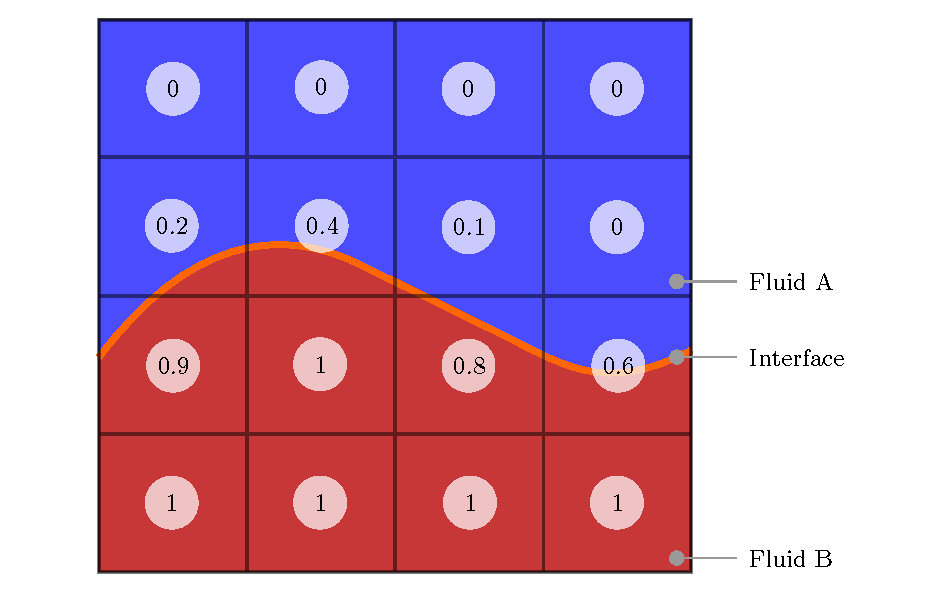
\includegraphics[width=0.68\textwidth]{images/vof.pdf}
    \captionof{figure}{Diagrama esquemático com o valor da fase $\alpha$ no respectivo volume finito.}
\end{frame}

\begin{frame}{Modelo bi-viscoso}
    Para baixas taxas de deformação, o material é modelado como um fluido de alta viscosidade, com valor constante $\eta_0$. Equação~\ref{eq:bi-viscous}.

    \begin{equation} \label{eq:bi-viscous}
        \eta = min \left( \eta_0 \hspace{0.2cm} , \hspace{0.2cm} \frac{\tau_0}{\shearrate} + K\shearrate^{n-1}  \right)
    \end{equation}

\end{frame}

% \begin{frame}{Geração das Geometrias}
%     \begin{minipage}[c]{0.55\textwidth}
%         \centering
%         \includegraphics[width=\textwidth]{../dissertation-project/fig/diagrams/stl_python.png}
%         \captionof{figure}{Algoritmo de geração das geometrias.}
%     \end{minipage}
%     \hfill
%     \begin{minipage}[c]{0.43\textwidth}
%         \begin{exampleblock}{Etapas}
%             \begin{enumerate}
%                 \item Vértices frontais, sem obstáculo; \pause
%                 \item Dimensões e quantidade de obstáculos a serem inseridos; \pause
%                 \item Inserir obstáculo conforme a forma; \pause
%                 \item Vértices posteriores; \pause
%                 \item Criação das faces (nomenclatura); \pause
%                 \item Geração dos arquivos em STL.
%             \end{enumerate}
%         \end{exampleblock}
%     \end{minipage}
%     \end{frame}


\begin{frame}{Geometria}
    \begin{minipage}[c]{0.58\textwidth}
        \includegraphics[width=\textwidth]{../dissertation-project/fig/svgs/geometry.pdf}
    \end{minipage}
    \hfill
    \begin{minipage}[c]{0.38\textwidth}
        \captionof{figure}{
            Exemplos das geometrias (canais) geradas para cada tipo de obstáculo.\\ 
            (a) Obstáculo retangular.\\ 
            (b) Obstáculo triangular.\\ 
            (c) Obstáculo semicircular.}
    \end{minipage}
\end{frame}


% \begin{frame}{Condições de Contorno}
%     \begin{minipage}[c]{0.45\textwidth}
%             \begin{table}[ht]
%                 \centering
%                 \caption{Condições de Contorno para a geometria inicial proposta.}
%                 \scriptsize
%                 \begin{tabular}{llll}
%                 \toprule
%                 Boundary                                                                       & Field    & Type      & Value \\ 
%                 \midrule
%                 \multirow{3}{*}{Inlet}                                                         & $\alpha$ & Dirichlet & $ \alpha = 1 $                                   \\ 
%                                                                                                & $p$      & Neumann   & $\bm{n} \cdot \nabla p = 0 $                     \\  
%                                                                                                & $U$      & Dirichlet & $ u = u_0 $                                      \\ 
%                 \midrule
%                 \multirow{3}{*}{Outlet}                                                        & $\alpha$ & Dirichlet & $ \alpha = 1 $                                   \\ 
%                                                                                                & $p$      & Dirichlet & $ p = 0 $                                        \\  
%                                                                                                & $U$      & Neumann   & $\bm{n} \cdot \nabla \velvector = 0 $            \\
%                 \midrule
%                 \multirow{3}{*}{Obstacle}                                                      & $\alpha$ & Neumann   & $ \alpha = 0 $                                   \\ 
%                                                                                                & $p$      & Neumann   & $\bm{n} \cdot \nabla p = 0 $                     \\  
%                                                                                                & $U$      & Dirichlet & $ u(y=0) = 0 $                                   \\
%                 \midrule
%                 \multirow{3}{*}{\begin{tabular}[c]{@{}l@{}}Walls,\\ Bottom Walls\end{tabular}} & $\alpha$ & Neumann   & $ \alpha = 0 $                                   \\ 
%                                                                                                & $p$      & Neumann   & $ \bm{n} \cdot \nabla p = 0 $                    \\  
%                                                                                                & $U$      & Dirichlet & $ u(y=0) = 0 $                                   \\
%                 \bottomrule
%                 \end{tabular} \label{tab:boundary_conditions}
%                 \end{table}
%     \end{minipage}
%     \hfill
%     \begin{minipage}[c]{0.50\textwidth}
%         \centering
%         \includegraphics[width=\textwidth]{../dissertation-project/fig/png/bc_paraview.png}
%         \captionof{figure}{Condições de Contorno.}
%     \end{minipage}
% \end{frame}

\begin{frame}{Malha Numérica}
    \begin{minipage}[c]{0.68\textwidth}
        \includegraphics[width=\textwidth]{../dissertation-project/fig/svgs/mesh.pdf}
    \end{minipage}
    \hfill
    \begin{minipage}[c]{0.30\textwidth}
        \captionof{figure}{
            Malha numérica do canal com obstáculo semicircular. Destaque para o
            maior nível de refinamento no obstáculo, nas paredes adjacentes ao 
            obstáculo e na região de superfície livre do escoamento.}
    \end{minipage}
\end{frame}

\section{Cronograma}

\section{Cronograma}

\begin{frame}
    \centering
    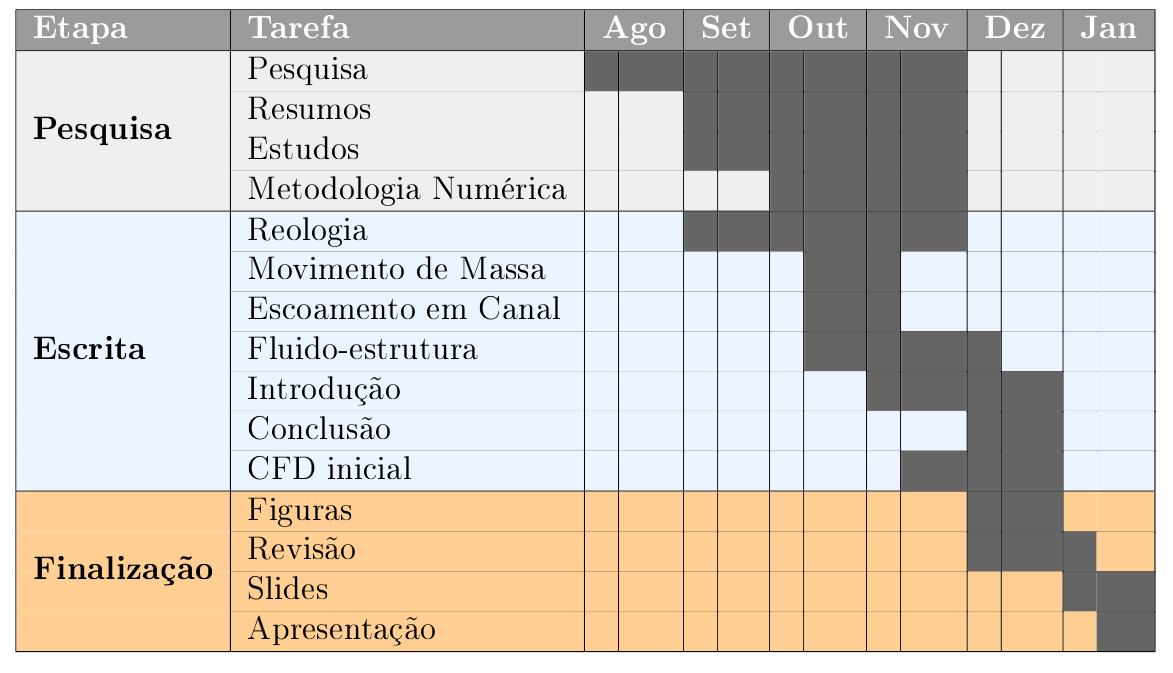
\includegraphics[width=0.8\textwidth]{images/cronograma.png}
\end{frame}

\begin{frame}[allowframebreaks]
    \printbibliography
\end{frame}

\begin{frame}
    \begin{center}
        {\Huge Perguntas?}
    \end{center}
\end{frame}

\end{document}